%! Author = breandan
%! Date = 2/22/21

% Preamble
\documentclass[11pt]{article}

% Packages
\usepackage{amsfonts}
\usepackage{amsmath}
\usepackage{graphicx}
\usepackage{hyperref}
\usepackage{float}
\usepackage{pgfplots}
\usepgfplotslibrary{fillbetween}
\usepackage{filecontents}
\usepackage[pdf]{graphviz}
\usepackage{tikz}
\usepackage{natbib}

\usepackage{booktabs}
\usepackage{pifont}
\usepackage{fontawesome}

\newcommand{\wmark}{\textcolor{orange}{\ding{45}}}
\newcommand{\cmark}{\textcolor{green!80!black}{\ding{51}}}
\newcommand{\xmark}{\textcolor{red}{\ding{55}}}


\usepackage{multicol}
\usepackage{amssymb}

%% Table
%
%\newcolumntype{R}[2]{%
%    >{\adjustbox{angle=#1,lap=\width-(#2)}\bgroup}%
%  l%
%    <{\egroup}%
%}
%\newcommand*\rot{\multicolumn{1}{R{55}{1em}}}

% Document

\title{Learning to search for software artifacts}
\author{Breandan Considine, Xujie Si, Jin Guo}
\begin{document}
\maketitle

\section{Introduction}

Humans are adept information foraging agents. We can quickly find relevant information in a large corpus by recognizing and following textual landmarks. Software projects are composed of a variety of semi-structured documents containing many clues where relevant information may be found. In this work, we train a model to navigate and read software artifacts like source code and documentation, in order to facilitate common programming tasks such as code search, completion, or defect prediction.

%Our work broadly falls under the umbrella of text-based reinforcement learning. Prior literature falls under two categories: natural or formal language. Reinforcement learning (RL) in the natural domain typically focuses on question answering~\citep{buck2017ask, chen2019reinforcement}, or interactive text games~\citep{he2015deep,ammanabrolu2018playing,narasimhan2015language,guo2020interactive,ammanabrolu2020graph}. RL techniques have begun to show promising results for program synthesis~\citep{ellis2019write, johnson2020learning, chen2020program}. Our work falls at the intersection of these two domains.

Early work in program learning realized the importance of graph-based representations~\citep{allamanis2017learning}, however explicit graph construction requires extensive feature-engineering. More recent work in program synthesis has explored incorporating a terminal~\citep{ellis2019write}, graphical~\citep{walke2020learning} or other user interface to explore the space of valid programs, however do not consider the scope or variety of artifacts in a software project. Others have shown the feasibility of learning a local graph~\citep{johnson2020learning} from source code, but still require an explicit parser to form the initial graph and adaption in settings where style, terminology and document structure vary remains a challenge.


Imagine a newly-hired developer, who has programming experience, but no prior knowledge about a closed-source project. She receives access to the team's Git repository and is assigned her first ticket: Fix test broken by \texttt{0fb98be}. After locating the commit and becoming familiar with the code, she queries StackOverflow, discovers a relevant solution, copies the code into the project, makes a few edits, presses run, and the test passes.

In order to accomplish a similar task, an information-seeking agent must be able to explore a local database for information, construct a query, and search a remote database. Similar to a human developer, it might traverse the project to gather information, taking note of various keywords, APIs and design patterns. While traversing the project, the model constructs a project-specific knowledge graph, which it uses to locate other relevant artifacts written by authors who solved the same problem.

%\begin{figure*}
%  \centering
%  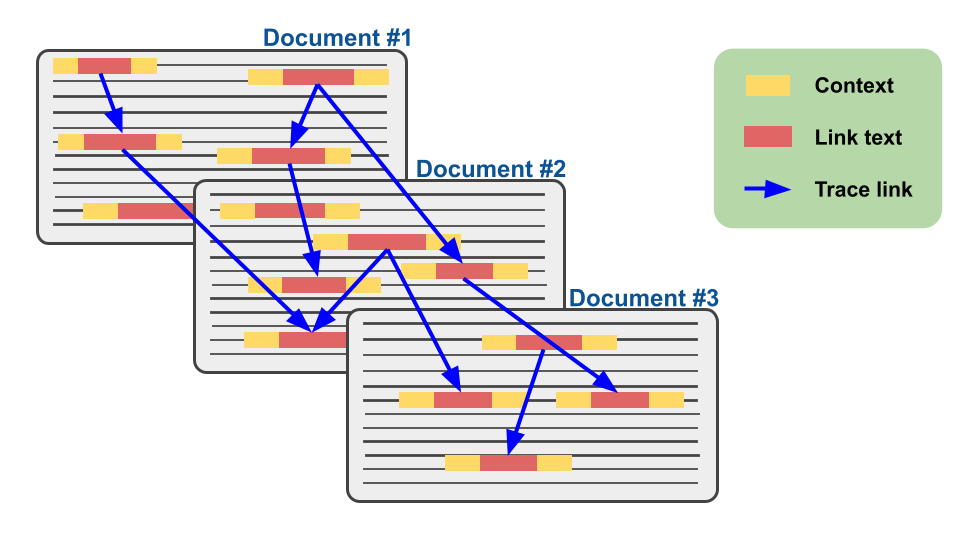
\includegraphics[width=0.8\textwidth]{use_graph}
%  \caption{Software projects consist of many documents which share common references. These references form an entity alignment graph, with vertices decorated by the surrounding context, and edges by the relation type, e.g. exact duplicate, fuzzy match or synthetic relation (learned or engineered).}
%\end{figure*}

%During evaluation, we measure task performance across search strategies. Depending on the task in question, various loss functions are possible, from a simple string distance metric over a masked code fragment, to more complex properties (e.g. the presence or absence of errors, or some internal state of the REPL) that must be satisfied by interacting with the runtime environment. Many program analysis and repair tasks are also possible, such as defect, duplicate or vulnerability detection and correction.

\section{Prior literature}

Prior work in the code search literature explores the text-to-code~\citep{husain2019codesearchnet} setting, where queries are typically considered to be a short sequence composed by the user, or code-to-code~\citep{kim2018facoy} setting where the query might be generated. Model performance typically evaluated using mean reciprocal rank (MRR), mean average precision (MAP), normalized discounted cumulative gain (NDCG), precision and recall at top N-results (P/R@N), or similar metrics. Although some~\citep{asyrofi2020ausearch} do incorporate other features from the local document, none however, consider the query in the context of a broader project. The ability to align contextual features from the surrounding project, we argue, is essential to delivering semantically relevant search results.

{ % begin box to localize effect of arraystretch change
\renewcommand{\arraystretch}{1.5}
\begin{table}[H]
  \small
  \begin{tabular}{lllc}
    Name & Type & Key contribution & Evaluation method \\
    \hline
    \href{https://github.com/breandan/gym-fs}{\textsc{Our Work}} & Project-to-code & Graph search & TBD \\
    \href{https://core.ac.uk/download/pdf/162022846.pdf#page=7}{\textsc{FaCoY}}~\citep{kim2018facoy} & Code-to-code & Similarity search & MRR \\
    \href{http://www.jameskoppel.com/files/papers/yogo-preprint.pdf#page=11}{\textsc{Yogo}}~\cite{premtoon2020semantic}     & Code-to-code & Equational reasoning & Case study \\
    \href{https://arxiv.org/pdf/1909.09436.pdf#page=5}{\textsc{CSNet}}~\citep{husain2019codesearchnet}     & Text-to-code & Big code benchmark & MRR \\
    \href{https://arxiv.org/pdf/1812.01158.pdf#section.5}{\textsc{Aroma}}~\citep{luan2019aroma}     & Code-to-code & Structural Search& Recall@N \\
    \href{https://raw.githubusercontent.com/mhilmiasyrofi/AUSearch/master/SANER_2020_AUSearch.pdf}{\textsc{AUSearch}}~\citep{asyrofi2020ausearch}     & Code-to-code & Type resolver & Highlight accuracy \\

    \href{https://arxiv.org/pdf/1905.03813.pdf#section.4}{\textsc{Cambronero}}~\citep{cambronero2019deep}     & Text-to-code & Semantics & Answered@N \\
    \href{https://guxd.github.io/papers/deepcs.pdf#section.5}{\textsc{DeepCS}}~\citep{gu2018deep}     & Text-to-code & Deep learning & FRank, *@N, MRR \\
  \end{tabular}
  \caption{\label{tab:ad_comparison} Comparison of existing code search tools.}
\end{table}
}

Although we draw some inspiration from the duplicate detection literature, their work presumes the code was intentionally duplicated or modified but is essentially identical in form or function. In contrast, our work seeks to help users discover artifacts which predictive of as-yet-incomplete code. By aligning salient features from the surrounding document and project graph, we approximate the notion of semantic similarity, without requring a language-specific parser like some methods~\citep{cambronero2019deep} do, and can more easily adapt to settings where the language and project structure varies.

Furthermore, unlike prior work, our work considers the surrounding project and related artifacts. Instead of parsing their contents explicitly, which may be computationally intractable, we allow the agent to construct the graph organically by exploring the filesystem, then extract a query.

\section{Method}

We fetch a dataset of repositories sampled repositories on GitHub, containing a mixture of filetypes representing source code and natural language artifacts. From each repository, we index all substrings of every line in every file using a variable height radix tree producing a multimap of $\texttt{kwdIndex: String -> List<Location<F, O>>}$ of $\texttt{String}$  queries to file-offset pairs. We also encode CodeBERT~\citep{feng2020codebert} sequence embeddings to substrings $\texttt{knnIndex: Vector -> Location<F, O>}$ using a Hierarchial Navigavble Small World Graph~\citep{malkov2018efficient} (HNSWG).


\begin{figure}[H]
  \centering
  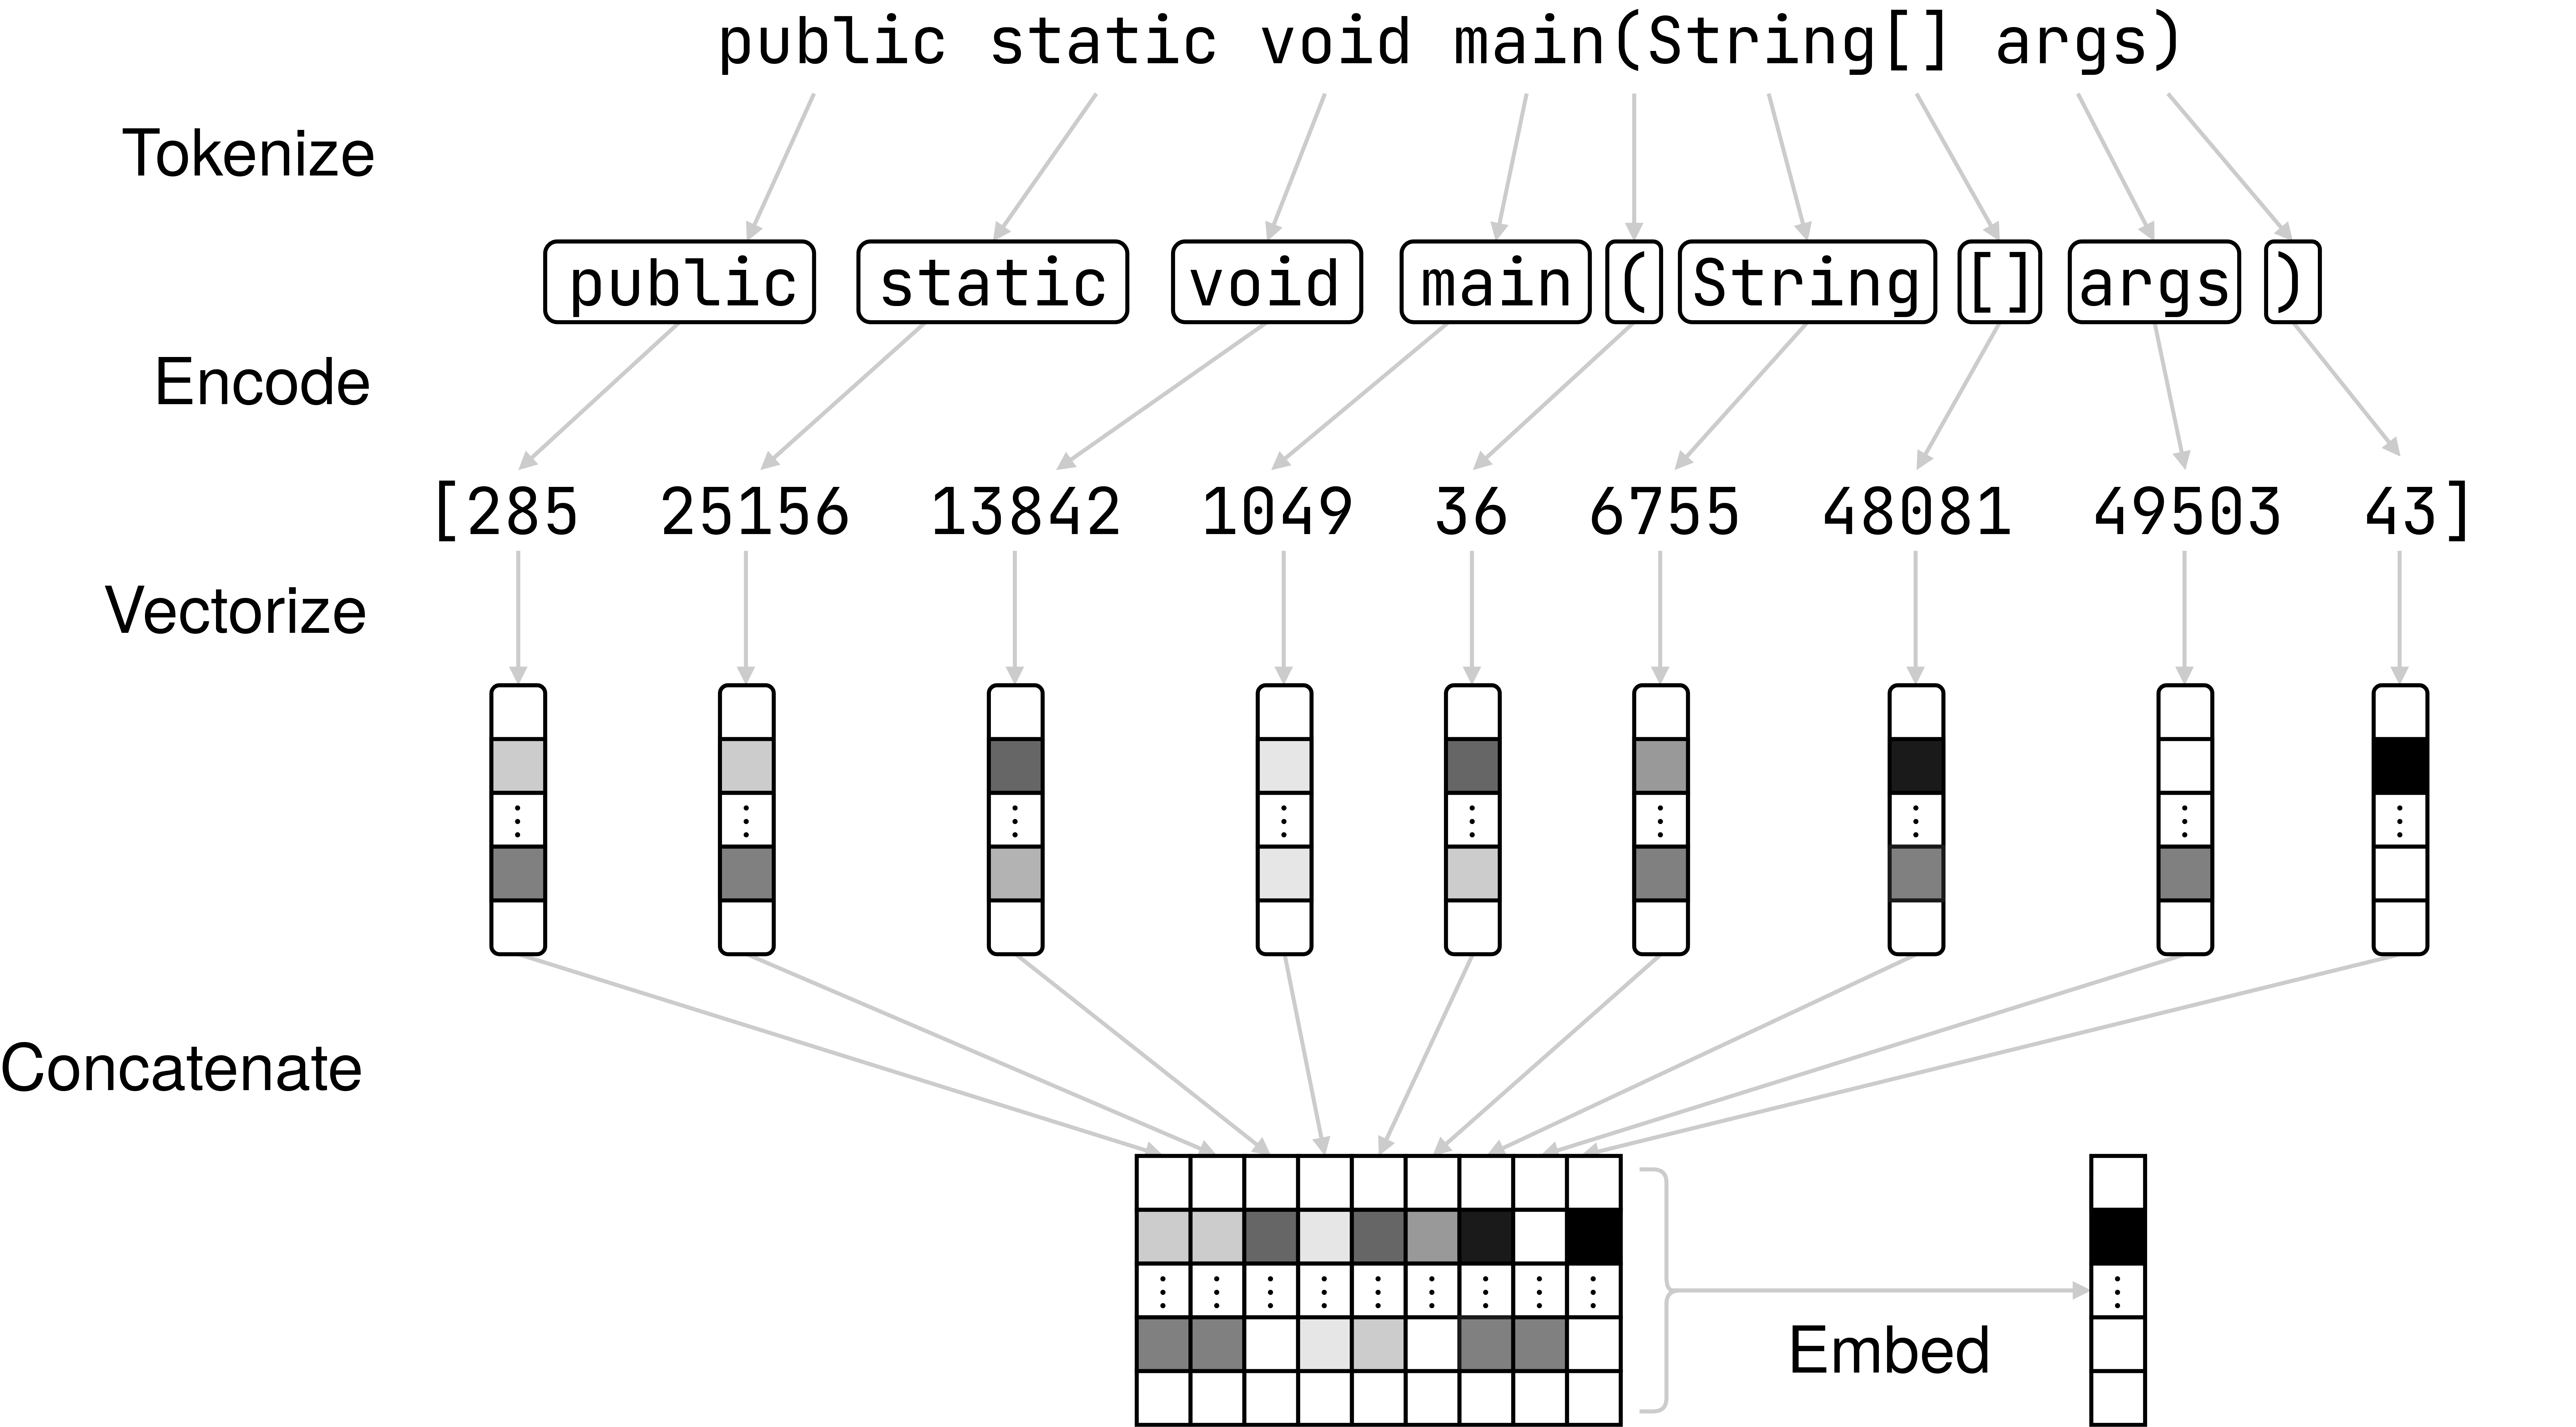
\includegraphics[width=0.85\textwidth]{bert_embedding}
  \caption{CodeBERT takes a unicode sequence and emits a vector sequence, which we accumulate into a single vector.}
  \label{fig:bert}
\end{figure}

For each token in a string, CodeBERT emits a length-768 vector, so a line with $n$ tokens produces a matrix of shape $\mathbb R^{768 \times (n + 1)}$, the first column of which contains the final hidden layer activations. We concatenate the CodeBERT sequence `\texttt{<s>}' and using the source tokens, encode and vectorize the encoded sequence using the vocabulary, then take the first row as our sequence embedding as depicted in Fig.~\ref{fig:bert}. In \S~\ref{sec:results}, we compare various distance-metrics to fetch the nearest sequence embeddings in our database and compare precision and recall across various types of distance metrics.

\begin{figure}[H]
  \centering
  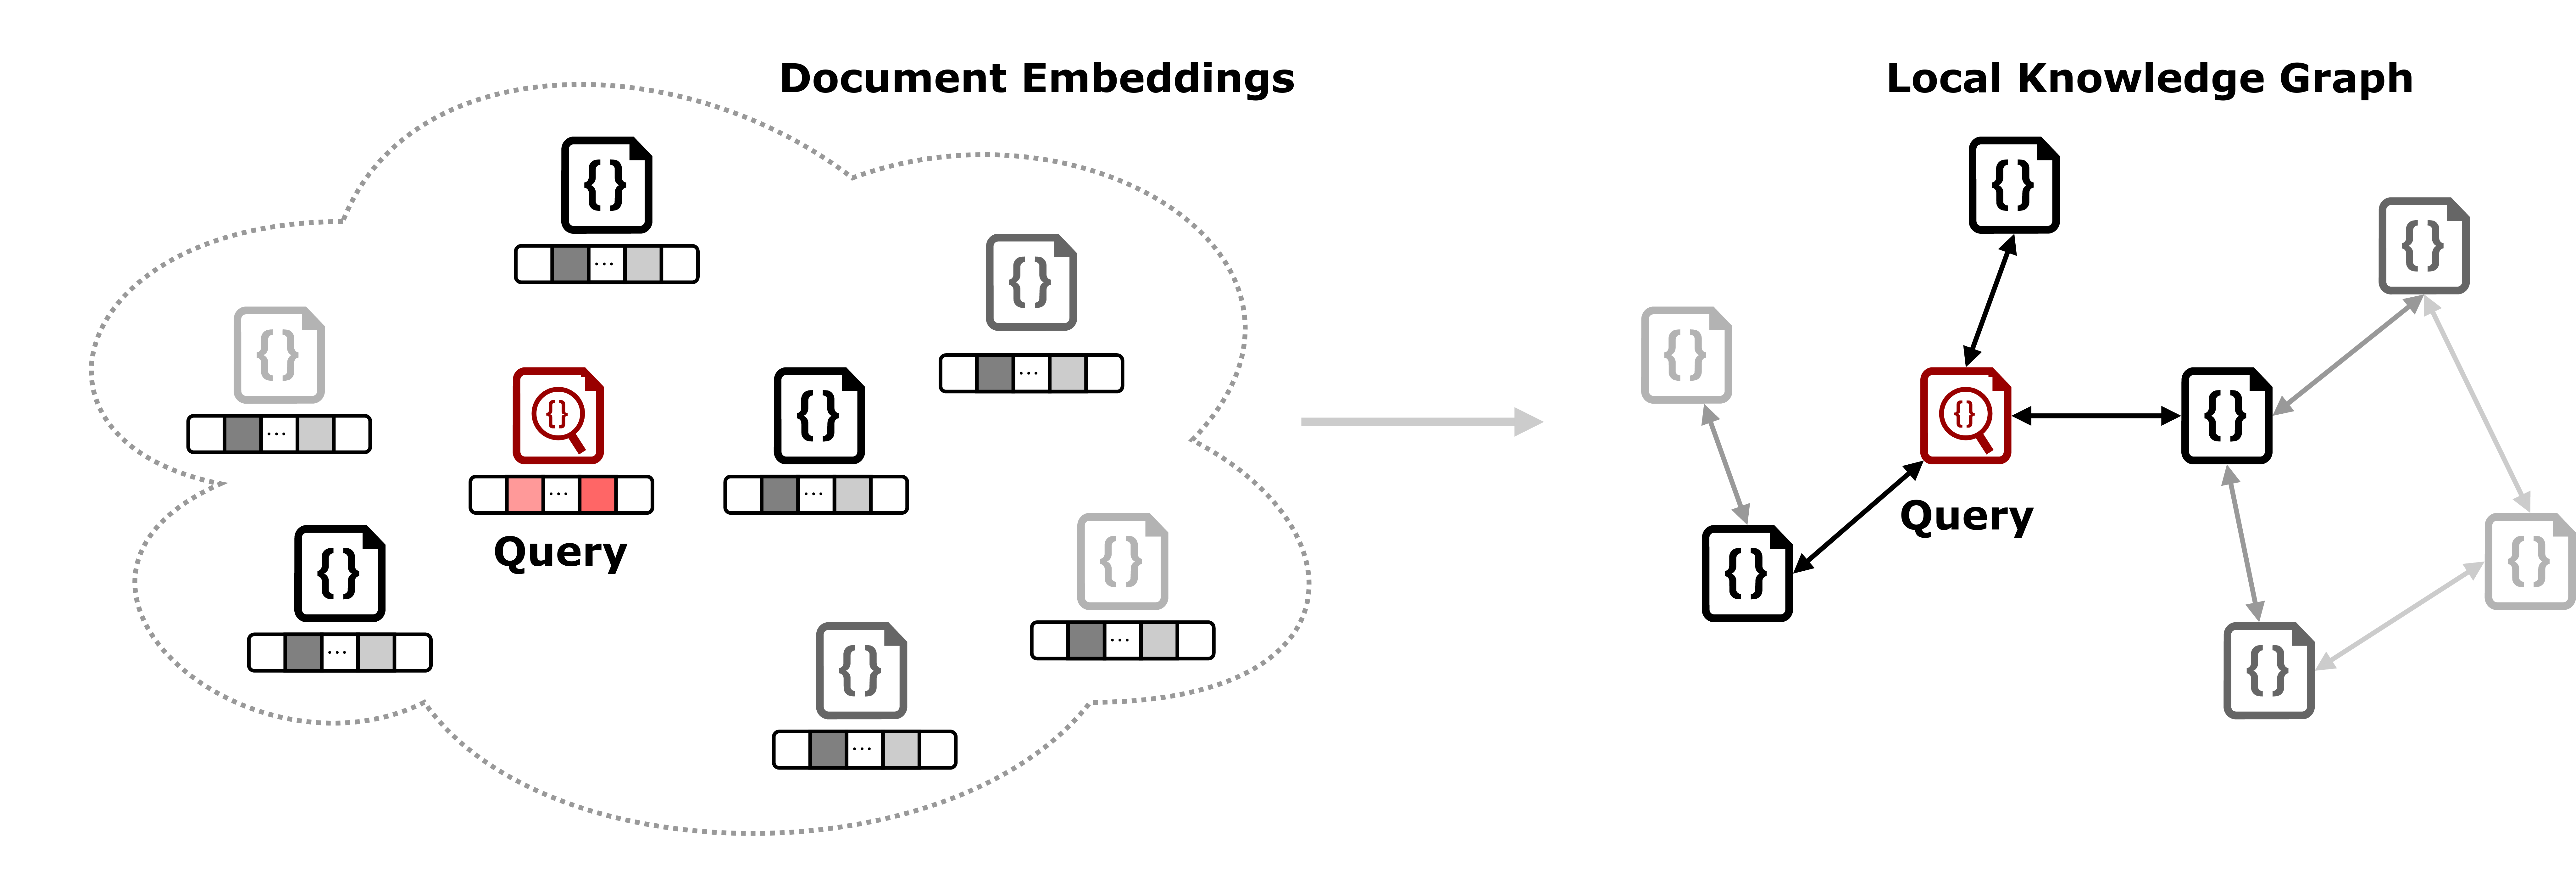
\includegraphics[width=\textwidth]{latent_kg}
  \caption{To compute our query neighborhood, we traverse the HNSWG up to max depth $d$, i.e. $d=1$ fetches the neighbors, $d=2$ fetches the neighbors-of-neighbors, and $d=3$ fetches the neighbors-of-neighbors-of-neighbors.}
  \label{fig:de2kg}
\end{figure}

For a given query and context, we first compute the context embedding and using a distance metric, fetch the k-nearest neighboring documents in latent space, forming the depth-1 nodes in our graph, then repeat this procedure recursively, pruning with a beam search heuristic based on the total path length in latent space. This procedure is depicted in Fig.~\ref{fig:de2kg}.

\begin{figure}[H]
  \centering
  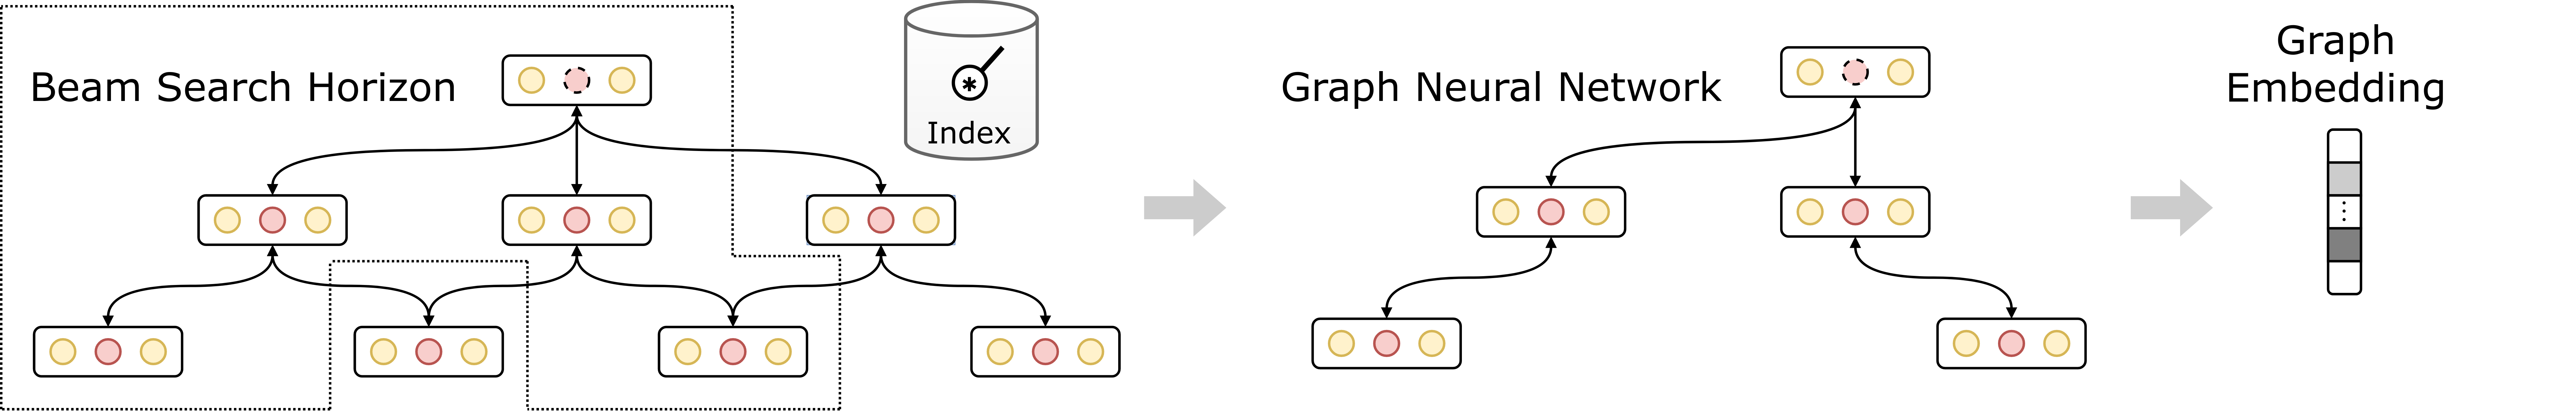
\includegraphics[width=1.05\textwidth]{architecture}
  \caption{Unlike language models which directly learn the data distribution, our model is designed to query an unseen database only available at test time. The model scores and selectively expands a subset of promising results within the database using a beam search heuristic, then runs message passing over the resulting graph to obtain the final task prediction.}
  \label{fig:architecture}
\end{figure}

Once the beam search procedure is complete, we have a graph representing the neighborhood of the nearest neighboring code fragments in the parent project. This forms a so-called \textit{virtual knowledge graph}, with nodes decorated by the CodeBERT sequence embeddings and edges decorated with the direction vector between documents. We then run $p$ rounds of message passing to obtain graph embedding or \textit{neighborhood summary vector} (Fig.~\ref{fig:architecture}).

% We initialize the policy network using a pretrained language model. Starting at the site of the prediction task and conditioning on its local context, the policy network draws K queries from its latent state, which are fed into the index to produce a set of matching locations. The model scores and selectively expands a subset of those locations, and the process is repeated using finite-horizon MCTS or similar beam search procedure to retrieve a set of contextually relevant locations within the parent project.
%
%The rollout traces form a graph of related locations inside each project and their corresponding context embeddings, which together form the GNN node features. Once the rollout ends, we run message passing on the resulting GNN for a fixed numbers of steps and decode the graph embedding to obtain a task prediction. The decoder, GNN parameters, and policy network are all trained end-to-end on the downstream task, e.g. code completion, defect detection or correction. After convergence, we compare the results across horizon size and analyze the queries and filetypes which are selected.

\section{Experiments}

In this work, we attempt to understand the relationship between entities in a software project. Our research seeks to answer the following questions:

\begin{enumerate}
  \item Which contexts in a software project share mutual information?
  \item To what degree can we claim the model has learned to:\begin{enumerate}
  \item Locate contextually relevant artifacts within a software project?
  \item Comprehend the semantic content of the artifacts traversed?
  \item Apply the knowledge gathered to perform the assigned task?
  \end{enumerate}
\end{enumerate}

In contrast with classical code completion models which only require a file-local context, our method is designed to navigate an entire project. In the following experiments, we compare completion accuracy with a vanilla sequence prediction model, as well as an AST-structured sequence prediction model trained from a corpus of Java projects on the same task.

We hypothesize that by jointly learning to choose locations in a project over which to attend while solving a downstream task, such as masked sequence completion, our model will produce a feature representation capable of locating and extracting information from semantically relevant contexts. We evaluate our hypothesis both qualitatively and quantitatively.

In our first set of experiments, we try to understand what is shared between sequences mapped to similar latent vectors. Do similar sequences share salient keywords? Are those keywords relevant to the task?

In our second experiment, we try to measure the information gain from including and excluding various filetypes through ablation. For graphs containing filetypes which include Markdown or Java, what kinds of information do these resources provide and which categories are most salient?

%In our third experiment, we compare prediction accuracy across architectures and datasets. Can we constrain the action space (e.g. only querying tokens from the surrounding context) for more efficient trajectory sampling, or allow arbitrary queries? How well does the model architecture transfer to new repositories, within and across programming languages?

In our third and final set of experiments, we compare performance across hyperparameters. Does contextual expansion lead to better task performence for a given sequence prediction task? By relaxing edge-construction criteria and increasing hyperparamers such as beam search budget, we would expect corresponding task performance to increase.

If our hypothesis is correct, the virtual knowledge graph will span both natural language and source code artifacts. If so, this would provide evidence to support the broader hypothesis~\citep{guo2017semantically} that documentation is a useful source of information. In addition to being useful for the prediction task itself, we anticipate our model could also be used for knowledge graph extraction and suggest semantically relevant code snippets to developers.

\section{Evaluation}

We evaluate on the following loss function, adapted from~\citep{husain2019codesearchnet}. Given a set of code and context pairs, $\mathbf{F} = (\mathbf{c}_i, \mathbf{d}_i)_{i = 1}^N$, where $\mathbf S \sim_{i.i.d.} \mathbf R_{d}$:

\begin{align}
  \mathcal{L} = \frac{1}{N}\sum_i^N \log\left(\frac{\left<\varphi(\mathbf{c}_i), \varphi(\mathbf{d}_i)\right>}{\sum_{j \neq i}^N \left<\varphi(\mathbf{c}_j), \varphi(\mathbf{d}_i)\right>}\right)
\end{align}

In other words, we minimize the distance between true code and context pairs, while maximizing the distance between distractors $(\mathbf c_j, \mathbf d_i)_{i \neq j}$.

%\section{Next steps}
%
%Our next steps are to build a simple environment which allows an agent to interact with a software repository and construct a graph. We will use an in-memory filesystem to store and load project artifacts. The policy network will need to be pretrained on a corpus of projects in the same language. To model the action space, we will use the radix tree of the parent project, with transition probabilities conditioned on the local context.
%
%For further details and to get started, please visit our GitHub page: \url{https://github.com/breandan/gym-fs}.

\section{Results}\label{sec:results}

Our preliminary results compare distance metrics (Fig.~\ref{fig:lev_vs_euclid}), explore embedding quality (Fig.~\ref{fig:embedding}) and visualize the synthetic knowledge graphs (Fig.~\ref{fig:graphs}).

\begin{figure}[H]
  \centering
  \begin{tikzpicture}[width]
    \begin{axis}[width=0.29\textwidth, height=0.3\textwidth, xlabel=Levenshtein, ylabel=Euclidean]
      \addplot table [mark=none,x=strdist, y=embdist, var=var, col sep=comma] {data/levenshtein.csv};

      \addplot [smooth, name path=upper,draw=none] table[x=strdist, y=embdist,var=var, y expr=\thisrow{embdist}+\thisrow{var}, col sep=comma] {data/levenshtein.csv};
      \addplot [smooth, name path=lower,draw=none] table[x=strdist, y=embdist,var=var, y expr=\thisrow{embdist}-\thisrow{var}, col sep=comma] {data/levenshtein.csv};
      \addplot [fill=red!10] fill between[of=upper and lower];
    \end{axis}
  \end{tikzpicture}
  \begin{tikzpicture}[width]
    \begin{axis}[width=0.29\textwidth, height=0.3\textwidth, xlabel=Damerau]
      \addplot table [mark=none,x=strdist, y=embdist, var=var, col sep=comma] {data/damerau.csv};

      \addplot [smooth, name path=upper,draw=none] table[x=strdist, y=embdist,var=var, y expr=\thisrow{embdist}+\thisrow{var}, col sep=comma] {data/damerau.csv};
      \addplot [smooth, name path=lower,draw=none] table[x=strdist, y=embdist,var=var, y expr=\thisrow{embdist}-\thisrow{var}, col sep=comma] {data/damerau.csv};
      \addplot [fill=red!10] fill between[of=upper and lower];
    \end{axis}
  \end{tikzpicture}
  \begin{tikzpicture}[width]
    \begin{axis}[width=0.29\textwidth, height=0.3\textwidth, xlabel=MetricLCS]
      \addplot table [mark=none,x=strdist, y=embdist, var=var, col sep=comma] {data/metriclcs.csv};

      \addplot [smooth, name path=upper,draw=none] table[x=strdist, y=embdist,var=var, y expr=\thisrow{embdist}+\thisrow{var}, col sep=comma] {data/metriclcs.csv};
      \addplot [smooth, name path=lower,draw=none] table[x=strdist, y=embdist,var=var, y expr=\thisrow{embdist}-\thisrow{var}, col sep=comma] {data/metriclcs.csv};
      \addplot [fill=red!10] fill between[of=upper and lower];
    \end{axis}
  \end{tikzpicture}
  \begin{tikzpicture}[width]
    \begin{axis}[width=0.29\textwidth, height=0.3\textwidth, xlabel=Jaccard]
      \addplot table [mark=none,x=strdist, y=embdist, var=var, col sep=comma] {data/jaccard.csv};

      \addplot [smooth, name path=upper,draw=none] table[x=strdist, y=embdist,var=var, y expr=\thisrow{embdist}+\thisrow{var}, col sep=comma] {data/jaccard.csv};
      \addplot [smooth, name path=lower,draw=none] table[x=strdist, y=embdist,var=var, y expr=\thisrow{embdist}-\thisrow{var}, col sep=comma] {data/jaccard.csv};
      \addplot [fill=red!10] fill between[of=upper and lower];
    \end{axis}
  \end{tikzpicture}
  \caption{CodeBERT latent space distance correlates with string distance.}
  \label{fig:lev_vs_euclid}
\end{figure}

\begin{figure}[H]
  \centering
  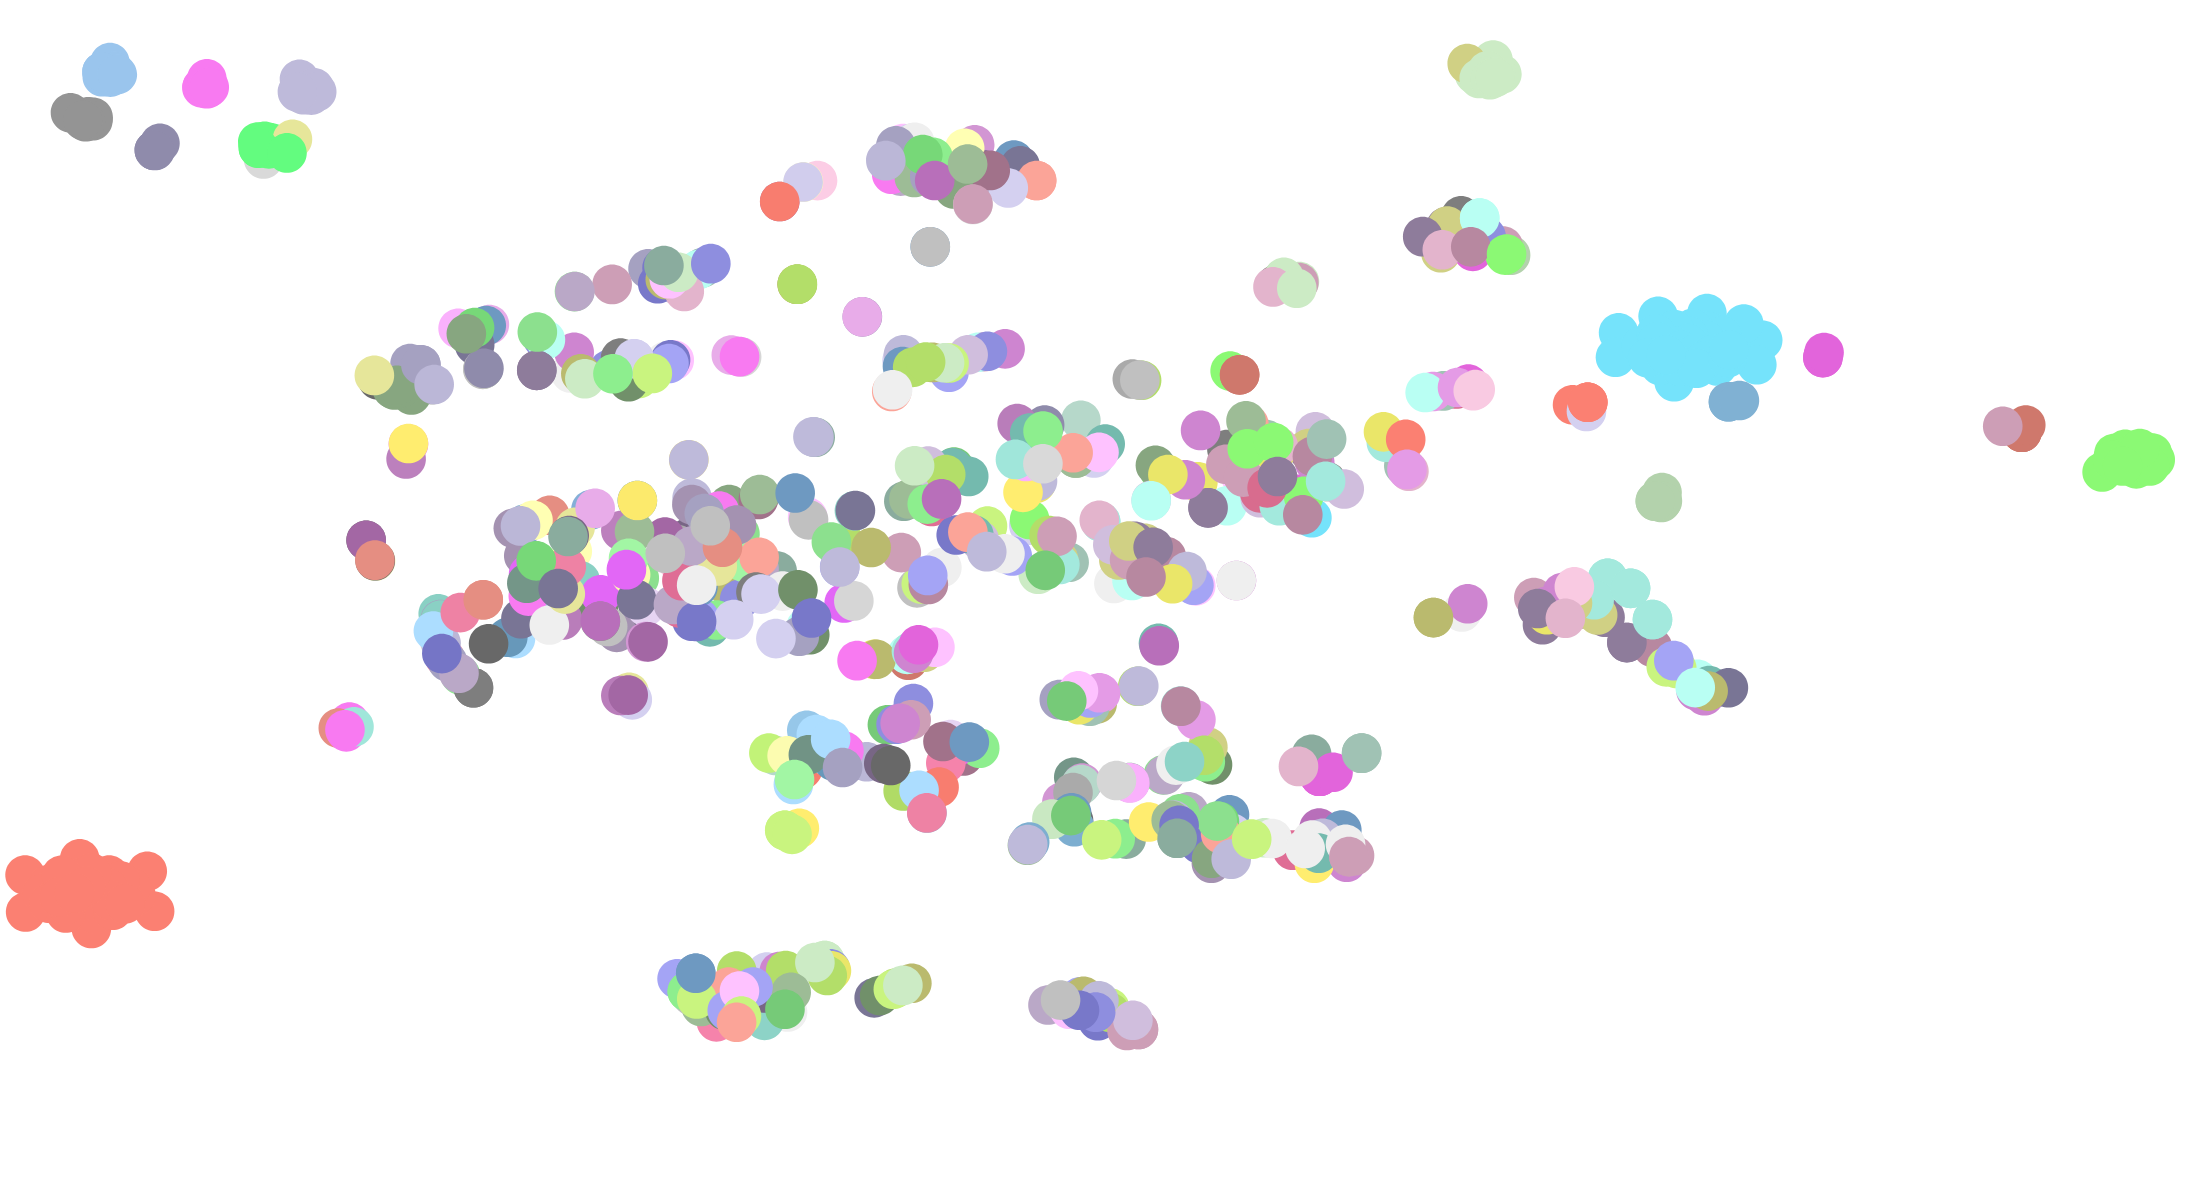
\includegraphics[width=0.4\textwidth]{embeddings}
  \caption{Reduced dimensionality TNSE embeddings colored by line length.}
  \label{fig:embedding}
\end{figure}

\begin{figure}[H]
  \centering
\resizebox{.2\textwidth}{!}{\includedot{data/query4}}
\resizebox{.2\textwidth}{!}{\includedot{data/query5}}
\resizebox{.2\textwidth}{!}{\includedot{data/query6}}
\resizebox{.2\textwidth}{!}{\includedot{data/query7}}
\resizebox{.2\textwidth}{!}{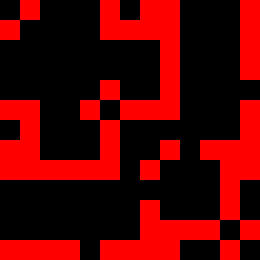
\includegraphics{data/context4}}
\resizebox{.2\textwidth}{!}{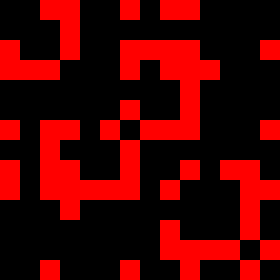
\includegraphics{data/context5}}
\resizebox{.2\textwidth}{!}{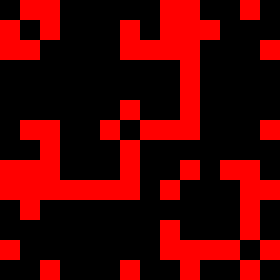
\includegraphics{data/context6}}
\resizebox{.2\textwidth}{!}{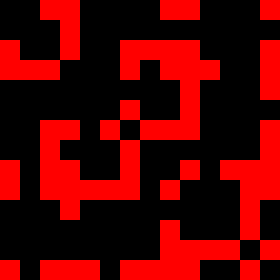
\includegraphics{data/context7}}
\caption{Example graphs sampled by beam search with $d=10, w=5$.}
\label{fig:graphs}
\end{figure}

  \bibliography{research_proposal}
  \bibliographystyle{plain}
%  \pagebreak
%  \appendix
%  \section{Appendix}
\end{document}